\documentclass[11p]{article}
% Packages
\usepackage{amsmath}
\usepackage{graphicx}
\usepackage[swedish]{babel}
\usepackage[
    backend=biber,
    style=authoryear-ibid,
    sorting=ynt
]{biblatex}
\usepackage[utf8]{inputenc}
\usepackage[T1]{fontenc}
%Källor
\addbibresource{mall.bib}
\graphicspath{ {./images/} }

\title{PMmall \\ \small Fysik 1}
\author{Magnus Silverdal }
\date{\today}

\begin{document}

\maketitle

\section{Referenser}
Referenser i text kan skrivas på två sätt: Enligt \textcite{Jens} kan man använde två typer av referenser, inbäddade i texten eller efter ett fakta \parencite{Fraenkel}. Ett till test för att se hur det ser ut \parencite{fermi}.



\section{Annat som kan vara bra att veta}
Det är lätt att skriva matematik i \LaTeX

\begin{equation}
    F = G \frac{M m}{r^2}
    \label{grav}
\end{equation}

Ekvation (\ref{grav}) känner ni igen...

\subsection{En underrubrik}
\begin{figure}[!h]
            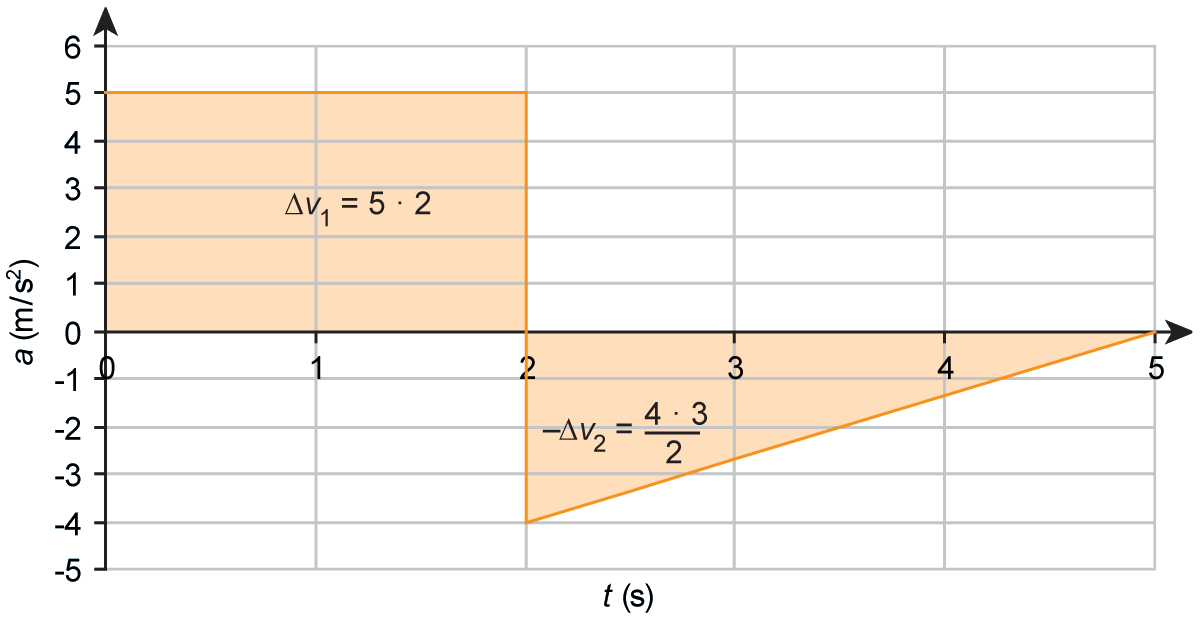
\includegraphics[width=0.8\textwidth]{accelerationTime.png}
            \caption{Acceleration-tid diagram. Källa: Impuls Fysik 1}
        \end{figure}
\printbibliography

\end{document}
